\documentclass[11pt,ignorenonframetext,]{beamer}
\setbeamertemplate{caption}[numbered]
\setbeamertemplate{caption label separator}{: }
\setbeamercolor{caption name}{fg=normal text.fg}
\beamertemplatenavigationsymbolsempty
\usepackage{lmodern}
\usepackage{amssymb,amsmath}
\usepackage{ifxetex,ifluatex}
\usepackage{fixltx2e} % provides \textsubscript
\ifnum 0\ifxetex 1\fi\ifluatex 1\fi=0 % if pdftex
  \usepackage[T1]{fontenc}
  \usepackage[utf8]{inputenc}
\else % if luatex or xelatex
  \ifxetex
    \usepackage{mathspec}
  \else
    \usepackage{fontspec}
  \fi
  \defaultfontfeatures{Ligatures=TeX,Scale=MatchLowercase}
\fi
\usetheme[]{metropolis}
% use upquote if available, for straight quotes in verbatim environments
\IfFileExists{upquote.sty}{\usepackage{upquote}}{}
% use microtype if available
\IfFileExists{microtype.sty}{%
\usepackage{microtype}
\UseMicrotypeSet[protrusion]{basicmath} % disable protrusion for tt fonts
}{}
\newif\ifbibliography
\hypersetup{
            pdftitle={Lecture 14},
            pdfauthor={Colin Rundel},
            pdfborder={0 0 0},
            breaklinks=true}
\urlstyle{same}  % don't use monospace font for urls
\usepackage{color}
\usepackage{fancyvrb}
\newcommand{\VerbBar}{|}
\newcommand{\VERB}{\Verb[commandchars=\\\{\}]}
\DefineVerbatimEnvironment{Highlighting}{Verbatim}{commandchars=\\\{\}}
% Add ',fontsize=\small' for more characters per line
\newenvironment{Shaded}{}{}
\newcommand{\KeywordTok}[1]{\textcolor[rgb]{0.00,0.44,0.13}{\textbf{#1}}}
\newcommand{\DataTypeTok}[1]{\textcolor[rgb]{0.56,0.13,0.00}{#1}}
\newcommand{\DecValTok}[1]{\textcolor[rgb]{0.25,0.63,0.44}{#1}}
\newcommand{\BaseNTok}[1]{\textcolor[rgb]{0.25,0.63,0.44}{#1}}
\newcommand{\FloatTok}[1]{\textcolor[rgb]{0.25,0.63,0.44}{#1}}
\newcommand{\ConstantTok}[1]{\textcolor[rgb]{0.53,0.00,0.00}{#1}}
\newcommand{\CharTok}[1]{\textcolor[rgb]{0.25,0.44,0.63}{#1}}
\newcommand{\SpecialCharTok}[1]{\textcolor[rgb]{0.25,0.44,0.63}{#1}}
\newcommand{\StringTok}[1]{\textcolor[rgb]{0.25,0.44,0.63}{#1}}
\newcommand{\VerbatimStringTok}[1]{\textcolor[rgb]{0.25,0.44,0.63}{#1}}
\newcommand{\SpecialStringTok}[1]{\textcolor[rgb]{0.73,0.40,0.53}{#1}}
\newcommand{\ImportTok}[1]{#1}
\newcommand{\CommentTok}[1]{\textcolor[rgb]{0.38,0.63,0.69}{\textit{#1}}}
\newcommand{\DocumentationTok}[1]{\textcolor[rgb]{0.73,0.13,0.13}{\textit{#1}}}
\newcommand{\AnnotationTok}[1]{\textcolor[rgb]{0.38,0.63,0.69}{\textbf{\textit{#1}}}}
\newcommand{\CommentVarTok}[1]{\textcolor[rgb]{0.38,0.63,0.69}{\textbf{\textit{#1}}}}
\newcommand{\OtherTok}[1]{\textcolor[rgb]{0.00,0.44,0.13}{#1}}
\newcommand{\FunctionTok}[1]{\textcolor[rgb]{0.02,0.16,0.49}{#1}}
\newcommand{\VariableTok}[1]{\textcolor[rgb]{0.10,0.09,0.49}{#1}}
\newcommand{\ControlFlowTok}[1]{\textcolor[rgb]{0.00,0.44,0.13}{\textbf{#1}}}
\newcommand{\OperatorTok}[1]{\textcolor[rgb]{0.40,0.40,0.40}{#1}}
\newcommand{\BuiltInTok}[1]{#1}
\newcommand{\ExtensionTok}[1]{#1}
\newcommand{\PreprocessorTok}[1]{\textcolor[rgb]{0.74,0.48,0.00}{#1}}
\newcommand{\AttributeTok}[1]{\textcolor[rgb]{0.49,0.56,0.16}{#1}}
\newcommand{\RegionMarkerTok}[1]{#1}
\newcommand{\InformationTok}[1]{\textcolor[rgb]{0.38,0.63,0.69}{\textbf{\textit{#1}}}}
\newcommand{\WarningTok}[1]{\textcolor[rgb]{0.38,0.63,0.69}{\textbf{\textit{#1}}}}
\newcommand{\AlertTok}[1]{\textcolor[rgb]{1.00,0.00,0.00}{\textbf{#1}}}
\newcommand{\ErrorTok}[1]{\textcolor[rgb]{1.00,0.00,0.00}{\textbf{#1}}}
\newcommand{\NormalTok}[1]{#1}
\usepackage{longtable,booktabs}
\usepackage{caption}
% These lines are needed to make table captions work with longtable:
\makeatletter
\def\fnum@table{\tablename~\thetable}
\makeatother
\usepackage{graphicx,grffile}
\makeatletter
\def\maxwidth{\ifdim\Gin@nat@width>\linewidth\linewidth\else\Gin@nat@width\fi}
\def\maxheight{\ifdim\Gin@nat@height>\textheight0.8\textheight\else\Gin@nat@height\fi}
\makeatother
% Scale images if necessary, so that they will not overflow the page
% margins by default, and it is still possible to overwrite the defaults
% using explicit options in \includegraphics[width, height, ...]{}
\setkeys{Gin}{width=\maxwidth,height=\maxheight,keepaspectratio}

% Prevent slide breaks in the middle of a paragraph:
\widowpenalties 1 10000
\raggedbottom

\AtBeginPart{
  \let\insertpartnumber\relax
  \let\partname\relax
  \frame{\partpage}
}
\AtBeginSection{
  \ifbibliography
  \else
    \let\insertsectionnumber\relax
    \let\sectionname\relax
    \frame{\sectionpage}
  \fi
}
\AtBeginSubsection{
  \let\insertsubsectionnumber\relax
  \let\subsectionname\relax
  \frame{\subsectionpage}
}

\setlength{\parindent}{0pt}
\setlength{\parskip}{6pt plus 2pt minus 1pt}
\setlength{\emergencystretch}{3em}  % prevent overfull lines
\providecommand{\tightlist}{%
  \setlength{\itemsep}{0pt}\setlength{\parskip}{0pt}}
\setcounter{secnumdepth}{0}

\usepackage{geometry}
\usepackage{graphicx}
\usepackage{amssymb}
\usepackage{color}          	% gives color options
\usepackage{url}		% produces hyperlinks
\usepackage[english]{babel}
\usepackage{colortbl}	% allows for color usage in tables
\usepackage{multirow}	% allows for rows that span multiple rows in tables
\usepackage{xcolor}		% this package has a variety of color options
\usepackage{calc}
\usepackage{multicol}
\usepackage{wrapfig}
\usepackage{textcomp}
\usepackage{bm}
\usepackage{bbm}
\usepackage{setspace}
\usepackage{changepage}
\singlespacing

%%%%%%%%%%%%%%%%
% Small code output
%%%%%%%%%%%%%%%%

%% change fontsize of R code

\makeatletter
\@ifundefined{Shaded}{\newenvironment{Shaded}{}{}}{}
\makeatother


\let\oldShaded\Shaded
\let\endoldShaded\endShaded
\renewenvironment{Shaded}{\footnotesize\begin{spacing}{0.9}\oldShaded}{\endoldShaded\end{spacing}}

%% change fontsize of output
\let\oldverbatim\verbatim
\let\endoldverbatim\endverbatim
\renewenvironment{verbatim}{\footnotesize\begin{spacing}{0.9}\oldverbatim}{\endoldverbatim\end{spacing}}


\newcommand{\tinyoutput}{
  \renewenvironment{Shaded}{\tiny\begin{spacing}{0.9}\oldShaded}{\endoldShaded\end{spacing}}
  \renewenvironment{verbatim}{\tiny\begin{spacing}{0.9}\oldverbatim}{\endoldverbatim\end{spacing}}
}

\newcommand{\scriptoutput}{
  \renewenvironment{Shaded}{\scriptsize\begin{spacing}{0.9}\oldShaded}{\endoldShaded\end{spacing}}
  \renewenvironment{verbatim}{\scriptsize\begin{spacing}{0.9}\oldverbatim}{\endoldverbatim\end{spacing}}
}

\newcommand{\footnoteoutput}{
  \renewenvironment{Shaded}{\footnotesize\begin{spacing}{0.9}\oldShaded}{\endoldShaded\end{spacing}}
  \renewenvironment{verbatim}{\footnotesize\begin{spacing}{0.9}\oldverbatim}{\endoldverbatim\end{spacing}}
}

%\newcommand{\verbatimfont}[1]{\renewcommand{\verbatim@font}{\ttfamily#1}}


%%%%%%%%%%%%%%%%
% Custom Colors
%%%%%%%%%%%%%%%%

\xdefinecolor{oiBlue}{rgb}{0.15, 0.35, 0.55}
\xdefinecolor{gray}{rgb}{0.5, 0.5, 0.5}
\xdefinecolor{darkGray}{rgb}{0.3, 0.3, 0.3}
\xdefinecolor{darkerGray}{rgb}{0.2, 0.2, 0.2}
\xdefinecolor{rubineRed}{rgb}{0.89,0,0.30}
\xdefinecolor{linkCol}{rgb}{0.11,0.49,0.95}	
\xdefinecolor{irishGreen}{rgb}{0,0.60,0}	
\xdefinecolor{darkturquoise}{rgb}{0.44, 0.58, 0.86}
\definecolor{lightGreen}{rgb}{0.533,0.765,0.42}
%\xdefinecolor{hlblue}{rgb}{0.051,0.65,1}
\xdefinecolor{hlblue}{rgb}{ 0.055, 0.639, 0.831}
\definecolor{light}{rgb}{.337,.608,.741}
\definecolor{dark}{rgb}{.337,.608,.741}

\definecolor{cpink}{rgb}{0.93, 0.23, 0.51}

%%%%%%%%%%%%%%%%
% Custom Commands
%%%%%%%%%%%%%%%%

% text colors
\newcommand{\red}[1]{\textit{\textcolor{rubineRed}{#1}}}
\newcommand{\orange}[1]{\textit{\textcolor{orange}{#1}}}
\newcommand{\pink}[1]{\textit{\textcolor{rubineRed!90!white!50}{#1}}}
\newcommand{\green}[1]{\textit{\textcolor{irishGreen}{#1}}}
\newcommand{\blue}[1]{\textit{\textcolor{darkturquoise}{#1}}}
\newcommand{\light}[1]{\textcolor{light}{\textbf{#1}}}
\newcommand{\dark}[1]{\textcolor{dark}{#1}}
\newcommand{\gray}[1]{\textcolor{gray}{#1}}


% links: webURL, webLin, appLink
\newcommand{\webURL}[1]{\urlstyle{same}{\textit{\textcolor{linkCol}{\url{#1}}} }}
\newcommand{\webLink}[2]{\href{#1}{\textcolor{linkCol}{{#2}}}}
\newcommand{\appLink}[2]{\href{#1}{\textcolor{lightGreen!80!black!90}{{#2}}}}

% mail
\newcommand{\mail}[1]{\href{mailto:#1}{\textit{\textcolor{linkCol}{#1}}}}

% highlighting: hl, hlGr, mathhl
\newcommand{\hl}[1]{\textit{\textcolor{hlblue}{#1}}}
\newcommand{\hlGr}[1]{\textit{\textcolor{lightGreen}{#1}}}
\newcommand{\hlRd}[1]{\textit{\textcolor{rubineRed}{#1}}}
\newcommand{\mathhl}[1]{\textcolor{hlblue}{\ensuremath{#1}}}

% example
\newcommand{\ex}[1]{\textcolor{blue}{{{\small (#1)}}}}


\DeclareMathOperator*{\argmin}{arg\,min}
\DeclareMathOperator*{\argmax}{arg\,max}

\title{Lecture 14}
\subtitle{Full Posterior Pred \& Covariance Functions}
\author{Colin Rundel}
\date{03/06/2017}

\begin{document}
\frame{\titlepage}

\section{Full Posterior Predictive
Distribution}\label{full-posterior-predictive-distribution}

\begin{frame}{FRN Data}

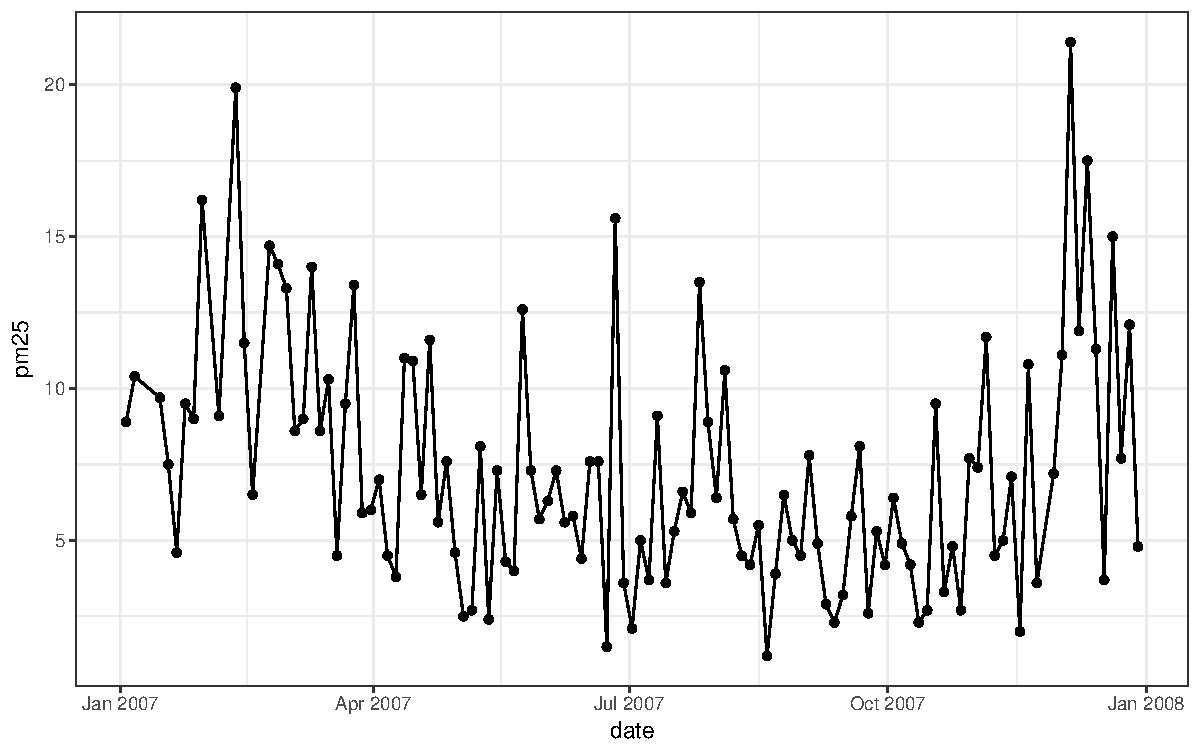
\includegraphics{Lec14_files/figure-beamer/unnamed-chunk-1-1.pdf}

\end{frame}

\begin{frame}[fragile]{JAGS Model}

\scriptoutput

\begin{verbatim}
## model{
##   y ~ dmnorm(mu, inverse(Sigma))
## 
##   for (i in 1:N) {
##     mu[i] = beta[1]+ beta[2] * x[i] + beta[3] * x[i]^2
##   }
##   
##   for (i in 1:(N-1)) {
##     for (j in (i+1):N) {
##       Sigma[i,j] = sigma2 * exp(- pow(l*d[i,j],2))
##       Sigma[j,i] = Sigma[i,j]
##     }
##   }
## 
##   for (k in 1:N) {
##     Sigma[k,k] = sigma2 + sigma2_w
##   }
## 
##   for (i in 1:3) {
##     beta[i] ~ dt(0, 2.5, 1)
##   }
##   sigma2_w ~ dnorm(10, 1/25) T(0,)
##   sigma2   ~ dnorm(10, 1/25) T(0,)
##   l        ~ dt(0, 2.5, 1) T(0,) 
## }
\end{verbatim}

\end{frame}

\begin{frame}{Posterior}

\begin{longtable}[]{@{}lrrrr@{}}
\toprule
param & post\_mean & post\_med & post\_lower &
post\_upper\tabularnewline
\midrule
\endhead
beta{[}1{]} & 9.2136151 & 11.4359371 & -0.4309078 &
15.2615892\tabularnewline
beta{[}2{]} & -0.0361357 & -0.0551308 & -0.1012205 &
0.0849476\tabularnewline
beta{[}3{]} & 0.0001007 & 0.0001367 & -0.0001924 &
0.0002552\tabularnewline
l & 0.8787410 & 0.0698553 & 0.0065124 & 7.0905582\tabularnewline
sigma2 & 8.4807746 & 7.8609848 & 1.5342164 & 18.6524860\tabularnewline
sigma2\_w & 9.7527513 & 10.4646243 & 2.2091857 &
14.8425142\tabularnewline
\bottomrule
\end{longtable}

\end{frame}

\begin{frame}[fragile,t]{Predicting}

\tinyoutput

\begin{Shaded}
\begin{Highlighting}[]
\NormalTok{l =}\StringTok{ }\NormalTok{post }\OperatorTok\StringTok{ }\KeywordTok{filter}\NormalTok{(param }\OperatorTok{==}\StringTok{ 'l'}\NormalTok{) }\OperatorTok\StringTok{ }\KeywordTok{select}\NormalTok{(post_med) }\OperatorTok\StringTok{ }\KeywordTok{unlist}\NormalTok{()}
\NormalTok{sigma2 =}\StringTok{ }\NormalTok{post }\OperatorTok\StringTok{ }\KeywordTok{filter}\NormalTok{(param }\OperatorTok{==}\StringTok{ 'sigma2'}\NormalTok{) }\OperatorTok\StringTok{ }\KeywordTok{select}\NormalTok{(post_med) }\OperatorTok\StringTok{ }\KeywordTok{unlist}\NormalTok{()}
\NormalTok{sigma2_w =}\StringTok{ }\NormalTok{post }\OperatorTok\StringTok{ }\KeywordTok{filter}\NormalTok{(param }\OperatorTok{==}\StringTok{ 'sigma2_w'}\NormalTok{) }\OperatorTok\StringTok{ }\KeywordTok{select}\NormalTok{(post_med) }\OperatorTok\StringTok{ }\KeywordTok{unlist}\NormalTok{()}

\NormalTok{beta0 =}\StringTok{ }\NormalTok{post }\OperatorTok\StringTok{ }\KeywordTok{filter}\NormalTok{(param }\OperatorTok{==}\StringTok{ 'beta[1]'}\NormalTok{) }\OperatorTok\StringTok{ }\KeywordTok{select}\NormalTok{(post_med) }\OperatorTok\StringTok{ }\KeywordTok{unlist}\NormalTok{()}
\NormalTok{beta1 =}\StringTok{ }\NormalTok{post }\OperatorTok\StringTok{ }\KeywordTok{filter}\NormalTok{(param }\OperatorTok{==}\StringTok{ 'beta[2]'}\NormalTok{) }\OperatorTok\StringTok{ }\KeywordTok{select}\NormalTok{(post_med) }\OperatorTok\StringTok{ }\KeywordTok{unlist}\NormalTok{()}
\NormalTok{beta2 =}\StringTok{ }\NormalTok{post }\OperatorTok\StringTok{ }\KeywordTok{filter}\NormalTok{(param }\OperatorTok{==}\StringTok{ 'beta[3]'}\NormalTok{) }\OperatorTok\StringTok{ }\KeywordTok{select}\NormalTok{(post_med) }\OperatorTok\StringTok{ }\KeywordTok{unlist}\NormalTok{()}

\NormalTok{reps=}\DecValTok{1000}

\NormalTok{x =}\StringTok{ }\NormalTok{pm25}\OperatorTok{$}\NormalTok{day}
\NormalTok{y =}\StringTok{ }\NormalTok{pm25}\OperatorTok{$}\NormalTok{pm25}
\NormalTok{x_pred =}\StringTok{ }\DecValTok{1}\OperatorTok{:}\DecValTok{365} \OperatorTok{+}\StringTok{ }\KeywordTok{rnorm}\NormalTok{(}\DecValTok{365}\NormalTok{, }\FloatTok{0.01}\NormalTok{)}

\NormalTok{mu =}\StringTok{ }\NormalTok{beta0 }\OperatorTok{+}\StringTok{ }\NormalTok{beta1}\OperatorTok{*}\NormalTok{x }\OperatorTok{+}\StringTok{ }\NormalTok{beta2}\OperatorTok{*}\NormalTok{x}\OperatorTok{^}\DecValTok{2}
\NormalTok{mu_pred =}\StringTok{ }\NormalTok{beta0 }\OperatorTok{+}\StringTok{ }\NormalTok{beta1}\OperatorTok{*}\NormalTok{x_pred }\OperatorTok{+}\StringTok{ }\NormalTok{beta2}\OperatorTok{*}\NormalTok{x_pred}\OperatorTok{^}\DecValTok{2}

\NormalTok{dist_o =}\StringTok{ }\KeywordTok{rdist}\NormalTok{(x)}
\NormalTok{dist_p =}\StringTok{ }\KeywordTok{rdist}\NormalTok{(x_pred)}
\NormalTok{dist_op =}\StringTok{ }\KeywordTok{rdist}\NormalTok{(x, x_pred)}
\NormalTok{dist_po =}\StringTok{ }\KeywordTok{t}\NormalTok{(dist_op)}
  
\NormalTok{cov_o  =}\StringTok{ }\KeywordTok{sq_exp_cov}\NormalTok{(dist_o,  }\DataTypeTok{sigma2 =}\NormalTok{ sigma2, }\DataTypeTok{l =}\NormalTok{ l) }\OperatorTok{+}\StringTok{ }\KeywordTok{nugget_cov}\NormalTok{(dist_o, }\DataTypeTok{sigma2 =}\NormalTok{ sigma2_w)}
\NormalTok{cov_p  =}\StringTok{ }\KeywordTok{sq_exp_cov}\NormalTok{(dist_p,  }\DataTypeTok{sigma2 =}\NormalTok{ sigma2, }\DataTypeTok{l =}\NormalTok{ l) }\OperatorTok{+}\StringTok{ }\KeywordTok{nugget_cov}\NormalTok{(dist_p, }\DataTypeTok{sigma2 =}\NormalTok{ sigma2_w)}
\NormalTok{cov_op =}\StringTok{ }\KeywordTok{sq_exp_cov}\NormalTok{(dist_op, }\DataTypeTok{sigma2 =}\NormalTok{ sigma2, }\DataTypeTok{l =}\NormalTok{ l) }\OperatorTok{+}\StringTok{ }\KeywordTok{nugget_cov}\NormalTok{(dist_op, }\DataTypeTok{sigma2 =}\NormalTok{ sigma2_w)}
\NormalTok{cov_po =}\StringTok{ }\KeywordTok{sq_exp_cov}\NormalTok{(dist_po, }\DataTypeTok{sigma2 =}\NormalTok{ sigma2, }\DataTypeTok{l =}\NormalTok{ l) }\OperatorTok{+}\StringTok{ }\KeywordTok{nugget_cov}\NormalTok{(dist_po, }\DataTypeTok{sigma2 =}\NormalTok{ sigma2_w)}

\NormalTok{cond_cov =}\StringTok{ }\NormalTok{cov_p }\OperatorTok{-}\StringTok{ }\NormalTok{cov_po }\OperatorTok\StringTok{ }\KeywordTok{solve}\NormalTok{(cov_o) }\OperatorTok\StringTok{ }\NormalTok{cov_op}
\NormalTok{cond_mu  =}\StringTok{ }\NormalTok{mu_pred }\OperatorTok{+}\StringTok{ }\NormalTok{cov_po }\OperatorTok\StringTok{ }\KeywordTok{solve}\NormalTok{(cov_o) }\OperatorTok\StringTok{ }\NormalTok{(y }\OperatorTok{-}\StringTok{ }\NormalTok{mu)}
  
\NormalTok{pred =}\StringTok{ }\NormalTok{cond_mu }\OperatorTok\StringTok{ }\KeywordTok{matrix}\NormalTok{(}\DecValTok{1}\NormalTok{, }\DataTypeTok{ncol=}\NormalTok{reps) }\OperatorTok{+}\StringTok{ }\KeywordTok{t}\NormalTok{(}\KeywordTok{chol}\NormalTok{(cond_cov)) }\OperatorTok\StringTok{ }\KeywordTok{matrix}\NormalTok{(}\KeywordTok{rnorm}\NormalTok{(}\KeywordTok{length}\NormalTok{(x_pred)}\OperatorTok{*}\NormalTok{reps), }\DataTypeTok{ncol=}\NormalTok{reps)}

\NormalTok{pred_df =}\StringTok{ }\NormalTok{pred }\OperatorTok\StringTok{ }\KeywordTok{t}\NormalTok{() }\OperatorTok\StringTok{ }\KeywordTok{post_summary}\NormalTok{() }\OperatorTok\StringTok{ }\KeywordTok{mutate}\NormalTok{(}\DataTypeTok{day=}\NormalTok{x_pred)}
\end{Highlighting}
\end{Shaded}

\end{frame}

\begin{frame}{Predictions}

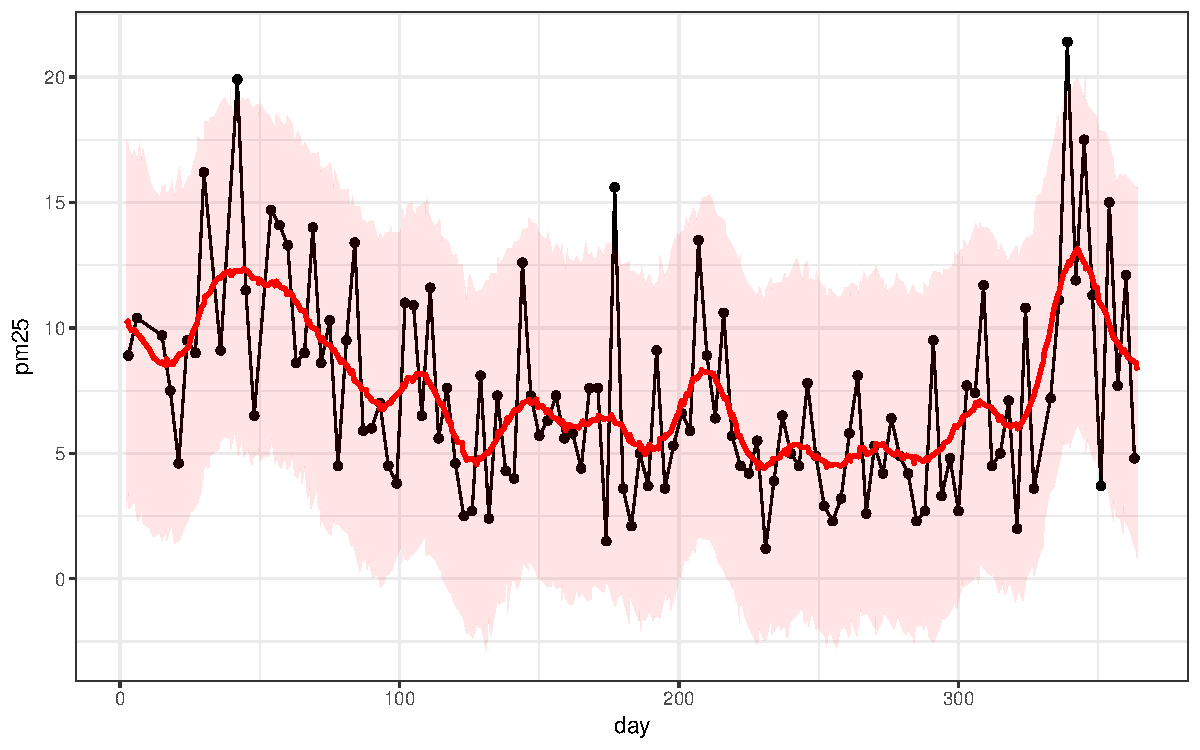
\includegraphics{Lec14_files/figure-beamer/unnamed-chunk-5-1.pdf}

\end{frame}

\begin{frame}[t]{Full Posterior Predictive Distribution}

Our posterior consists of samples from
\[ l, \sigma^2, \sigma^2_w, \beta_0, \beta_1, \beta_2 ~|~ \bm{y} \]

and for the purposes of generating the posterior predictions we sampled
\[ \bm{y}_{pred} ~|~ l^{(m)}, {\sigma^2}^{(m)}, {\sigma^2_w}^{(m)}, {\beta_0}^{(m)}, {\beta_1}^{(m)}, {\beta_2}^{(m)}, \bm{y} \]
where \(l^{(m)}\), etc. are the posterior median of that parameter.

\pause

\vspace{5mm}

In practice we should instead be sampling

\[ \bm{y}^{(i)}_{pred} ~|~ l^{(i)}, {\sigma^2}^{(i)}, {\sigma^2_w}^{(i)}, {\beta_0}^{(i)}, {\beta_1}^{(i)}, {\beta_2}^{(i)}, \bm{y} \]
since this takes into account the additional uncertainty in the model
parameters.

\end{frame}

\begin{frame}[fragile]{Full Posterior Predictive Distribution}

\tinyoutput

\begin{Shaded}
\begin{Highlighting}[]
\ControlFlowTok{if}\NormalTok{ (}\OperatorTok{!}\KeywordTok{file.exists}\NormalTok{(}\StringTok{"gp_pred.Rdata"}\NormalTok{))}
\NormalTok{\{}
\NormalTok{  x =}\StringTok{ }\NormalTok{pm25}\OperatorTok{$}\NormalTok{day; y =}\StringTok{ }\NormalTok{pm25}\OperatorTok{$}\NormalTok{pm25}
  
\NormalTok{  n_post_samp =}\StringTok{ }\KeywordTok{nrow}\NormalTok{(param)}
  
\NormalTok{  x_pred =}\StringTok{ }\DecValTok{1}\OperatorTok{:}\DecValTok{365} \OperatorTok{+}\StringTok{ }\KeywordTok{rnorm}\NormalTok{(}\DecValTok{365}\NormalTok{, }\FloatTok{0.01}\NormalTok{)}
\NormalTok{  y_pred =}\StringTok{ }\KeywordTok{matrix}\NormalTok{(}\OtherTok{NA}\NormalTok{, }\DataTypeTok{nrow=}\NormalTok{n_post_samp, }\DataTypeTok{ncol=}\KeywordTok{length}\NormalTok{(x_pred))}
  \KeywordTok{colnames}\NormalTok{(y_pred) =}\StringTok{ }\KeywordTok{paste0}\NormalTok{(}\StringTok{"Y_pred["}\NormalTok{, }\KeywordTok{round}\NormalTok{(x_pred,}\DecValTok{0}\NormalTok{), }\StringTok{"]"}\NormalTok{)}
  
  \ControlFlowTok{for}\NormalTok{(i }\ControlFlowTok{in} \DecValTok{1}\OperatorTok{:}\NormalTok{n_post_samp)}
\NormalTok{  \{}
\NormalTok{    l =}\StringTok{ }\NormalTok{param[i,}\StringTok{'l'}\NormalTok{]}
\NormalTok{    sigma2 =}\StringTok{ }\NormalTok{param[i,}\StringTok{'sigma2'}\NormalTok{]}
\NormalTok{    sigma2_w =}\StringTok{ }\NormalTok{param[i,}\StringTok{'sigma2_w'}\NormalTok{]}
\NormalTok{    beta0 =}\StringTok{ }\NormalTok{betas[i,}\StringTok{"beta[1]"}\NormalTok{]}
\NormalTok{    beta1 =}\StringTok{ }\NormalTok{betas[i,}\StringTok{"beta[2]"}\NormalTok{]}
\NormalTok{    beta2 =}\StringTok{ }\NormalTok{betas[i,}\StringTok{"beta[3]"}\NormalTok{]}
    
\NormalTok{    mu =}\StringTok{ }\NormalTok{beta0 }\OperatorTok{+}\StringTok{ }\NormalTok{beta1}\OperatorTok{*}\NormalTok{x }\OperatorTok{+}\StringTok{ }\NormalTok{beta2}\OperatorTok{*}\NormalTok{x}\OperatorTok{^}\DecValTok{2}
\NormalTok{    mu_pred =}\StringTok{ }\NormalTok{beta0 }\OperatorTok{+}\StringTok{ }\NormalTok{beta1}\OperatorTok{*}\NormalTok{x_pred }\OperatorTok{+}\StringTok{ }\NormalTok{beta2}\OperatorTok{*}\NormalTok{x_pred}\OperatorTok{^}\DecValTok{2}
    
\NormalTok{    dist_o =}\StringTok{ }\KeywordTok{rdist}\NormalTok{(x)}
\NormalTok{    dist_p =}\StringTok{ }\KeywordTok{rdist}\NormalTok{(x_pred)}
\NormalTok{    dist_op =}\StringTok{ }\KeywordTok{rdist}\NormalTok{(x, x_pred)}
\NormalTok{    dist_po =}\StringTok{ }\KeywordTok{t}\NormalTok{(dist_op)}
      
\NormalTok{    cov_o  =}\StringTok{ }\KeywordTok{sq_exp_cov}\NormalTok{(dist_o,  }\DataTypeTok{sigma2 =}\NormalTok{ sigma2, }\DataTypeTok{l =}\NormalTok{ l) }\OperatorTok{+}\StringTok{ }\KeywordTok{nugget_cov}\NormalTok{(dist_o,  }\DataTypeTok{sigma2 =}\NormalTok{ sigma2_w)}
\NormalTok{    cov_p  =}\StringTok{ }\KeywordTok{sq_exp_cov}\NormalTok{(dist_p,  }\DataTypeTok{sigma2 =}\NormalTok{ sigma2, }\DataTypeTok{l =}\NormalTok{ l) }\OperatorTok{+}\StringTok{ }\KeywordTok{nugget_cov}\NormalTok{(dist_p,  }\DataTypeTok{sigma2 =}\NormalTok{ sigma2_w)}
\NormalTok{    cov_op =}\StringTok{ }\KeywordTok{sq_exp_cov}\NormalTok{(dist_op, }\DataTypeTok{sigma2 =}\NormalTok{ sigma2, }\DataTypeTok{l =}\NormalTok{ l) }\OperatorTok{+}\StringTok{ }\KeywordTok{nugget_cov}\NormalTok{(dist_op, }\DataTypeTok{sigma2 =}\NormalTok{ sigma2_w)}
\NormalTok{    cov_po =}\StringTok{ }\KeywordTok{sq_exp_cov}\NormalTok{(dist_po, }\DataTypeTok{sigma2 =}\NormalTok{ sigma2, }\DataTypeTok{l =}\NormalTok{ l) }\OperatorTok{+}\StringTok{ }\KeywordTok{nugget_cov}\NormalTok{(dist_po, }\DataTypeTok{sigma2 =}\NormalTok{ sigma2_w)}
    
\NormalTok{    cond_cov =}\StringTok{ }\NormalTok{cov_p }\OperatorTok{-}\StringTok{ }\NormalTok{cov_po }\OperatorTok\StringTok{ }\KeywordTok{solve}\NormalTok{(cov_o) }\OperatorTok\StringTok{ }\NormalTok{cov_op}
\NormalTok{    cond_mu  =}\StringTok{ }\NormalTok{mu_pred }\OperatorTok{+}\StringTok{ }\NormalTok{cov_po }\OperatorTok\StringTok{ }\KeywordTok{solve}\NormalTok{(cov_o) }\OperatorTok\StringTok{ }\NormalTok{(y }\OperatorTok{-}\StringTok{ }\NormalTok{mu)}
      
\NormalTok{    y_pred[i,] =}\StringTok{ }\NormalTok{cond_mu }\OperatorTok{+}\StringTok{ }\KeywordTok{t}\NormalTok{(}\KeywordTok{chol}\NormalTok{(cond_cov)) }\OperatorTok\StringTok{ }\KeywordTok{matrix}\NormalTok{(}\KeywordTok{rnorm}\NormalTok{(}\KeywordTok{length}\NormalTok{(x_pred)), }\DataTypeTok{ncol=}\DecValTok{1}\NormalTok{)}
\NormalTok{  \}}
  
\NormalTok{  y_pred_df =}\StringTok{ }\NormalTok{y_pred }\OperatorTok\StringTok{ }\KeywordTok{post_summary}\NormalTok{() }\OperatorTok\StringTok{ }\KeywordTok{mutate}\NormalTok{(}\DataTypeTok{x_pred =} \KeywordTok{round}\NormalTok{(x_pred,}\DecValTok{0}\NormalTok{))}
  \KeywordTok{save}\NormalTok{(x_pred, y_pred, y_pred_df, }\DataTypeTok{file=}\StringTok{"gp_pred.Rdata"}\NormalTok{)}
\NormalTok{\} }\ControlFlowTok{else}\NormalTok{ \{}
  \KeywordTok{load}\NormalTok{(}\StringTok{"gp_pred.Rdata"}\NormalTok{)}
\NormalTok{\}}
\end{Highlighting}
\end{Shaded}

\end{frame}

\begin{frame}{Full Posterior Predictive Distribution - Plots}

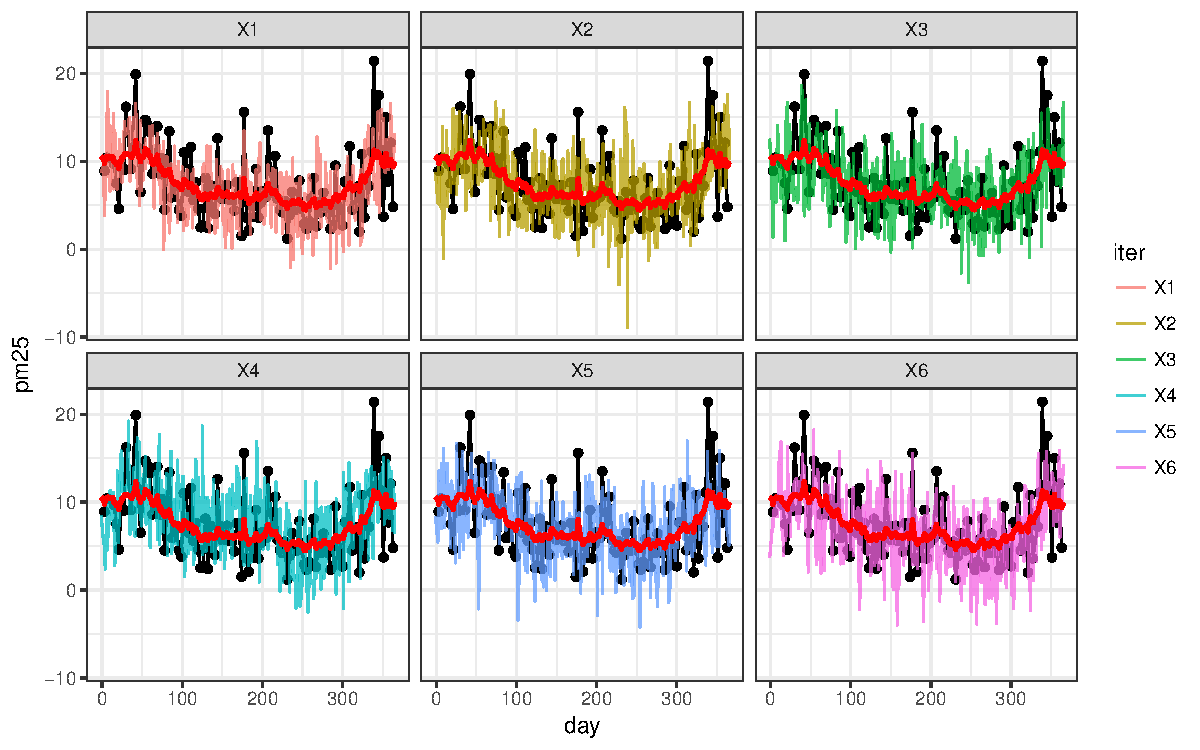
\includegraphics{Lec14_files/figure-beamer/unnamed-chunk-7-1.pdf}

\end{frame}

\begin{frame}{Full Posterior Predictive Distribution - Mean + CI}

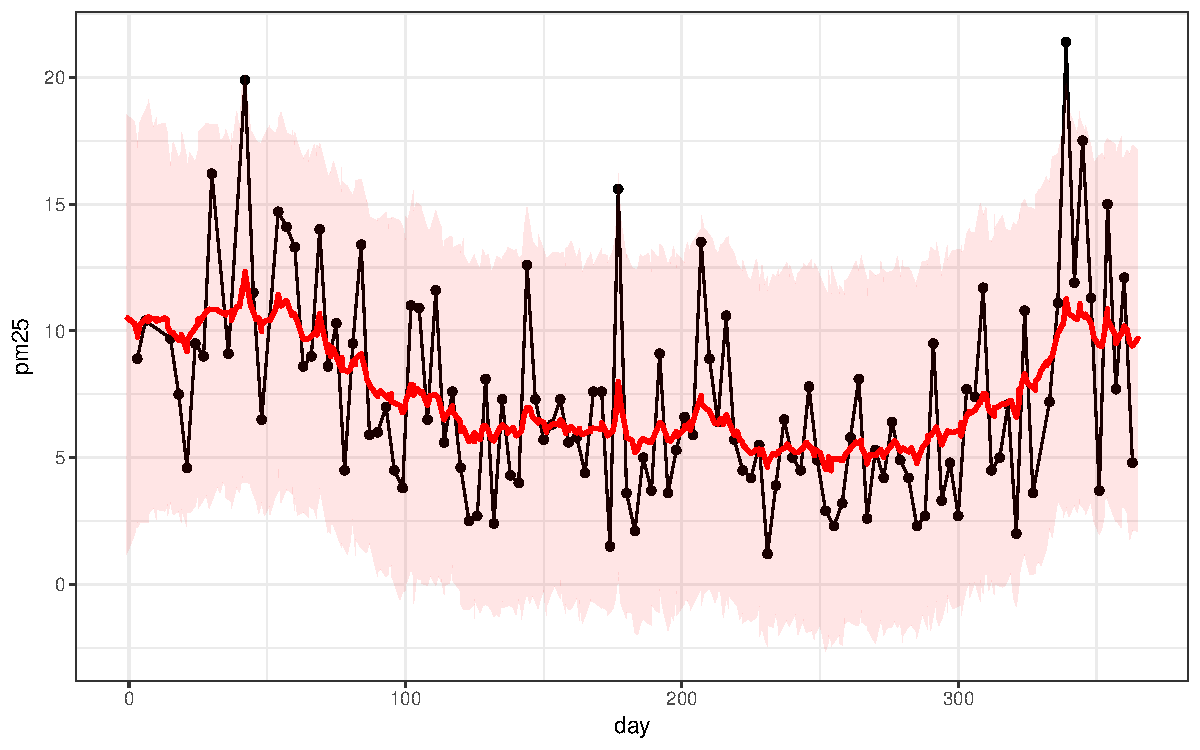
\includegraphics{Lec14_files/figure-beamer/unnamed-chunk-8-1.pdf}

\end{frame}

\section{More on Covariance
Functions}\label{more-on-covariance-functions}

\begin{frame}[t]{Nugget Covariance}

\[ Cov(y_{t_i}, y_{t_j}) = Cov(h = |t_i - t_j|) = \sigma^2 \mathbbm{1}_{\{h=0\}} \]

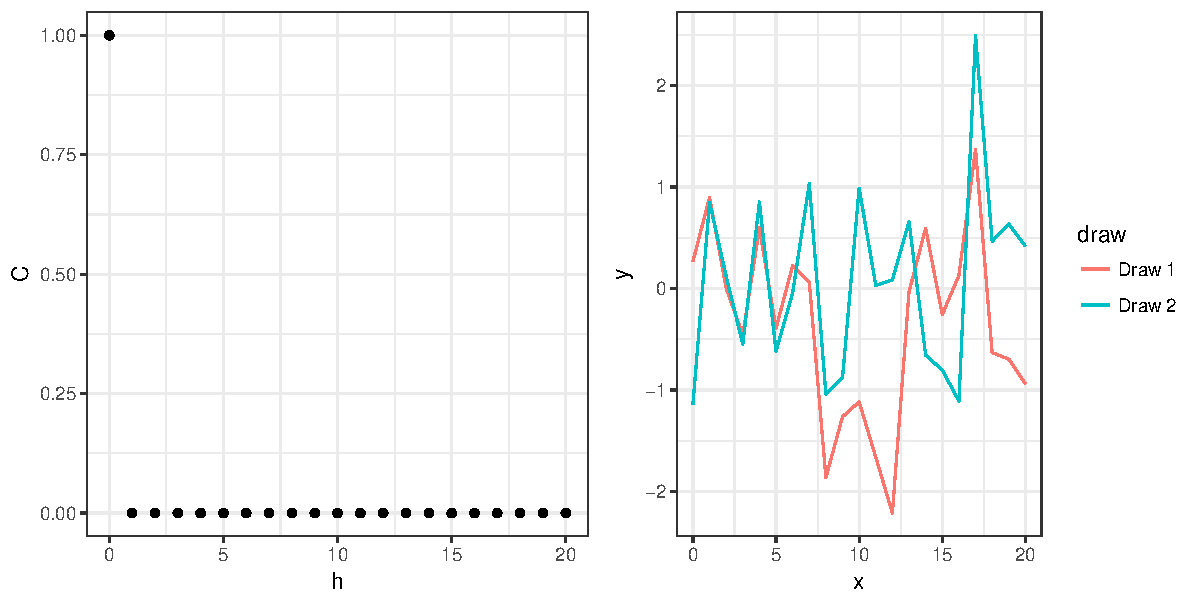
\includegraphics{Lec14_files/figure-beamer/unnamed-chunk-9-1.pdf}

\end{frame}

\begin{frame}[t]{(- / Power / Square) Exponential Covariance}

\vspace{-5mm}
\[ Cov(y_{t_i}, y_{t_j}) = Cov(h = |t_i - t_j|) = \sigma^2\exp\left(-(h\,l)^p\right) \]

\begin{center}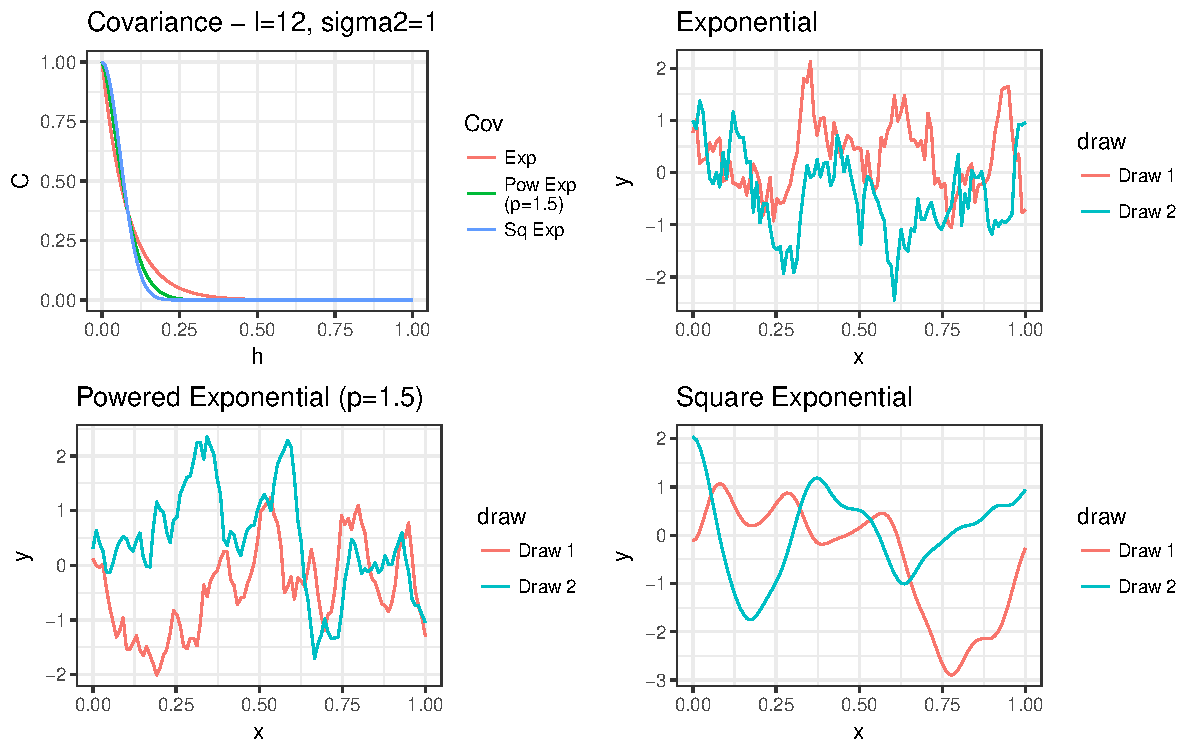
\includegraphics{Lec14_files/figure-beamer/unnamed-chunk-10-1} \end{center}

\end{frame}

\begin{frame}[t]{Matern Covariance}

\vspace{-10mm}
\[ Cov(y_{t_i}, y_{t_j}) = Cov(h = |t_i - t_j|) = \sigma^2 ~ \frac{2^{1-\nu}}{\Gamma(\nu)} ~ \left(\sqrt{2\nu}\, h \cdot l\right)^\nu ~ K_\nu\left(\sqrt{2\nu} \, h \cdot l\right)\]

\begin{center}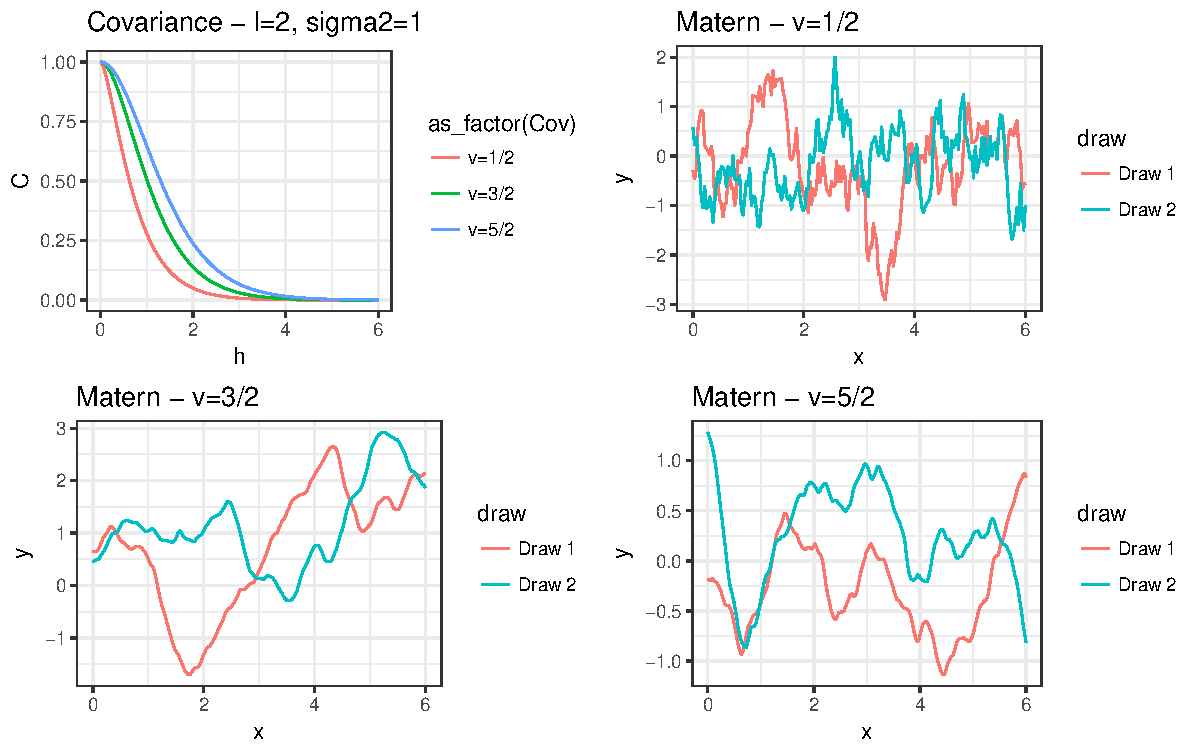
\includegraphics{Lec14_files/figure-beamer/unnamed-chunk-11-1} \end{center}

\end{frame}

\begin{frame}[t]{Rational Quadratic Covariance}

\vspace{-5mm}
\[ Cov(y_{t_i}, y_{t_j}) = Cov(h = |t_i - t_j|) = \sigma^2 \left(1 + \frac{h^2 \, l^2}{\alpha}\right)^{-\alpha}\]

\begin{center}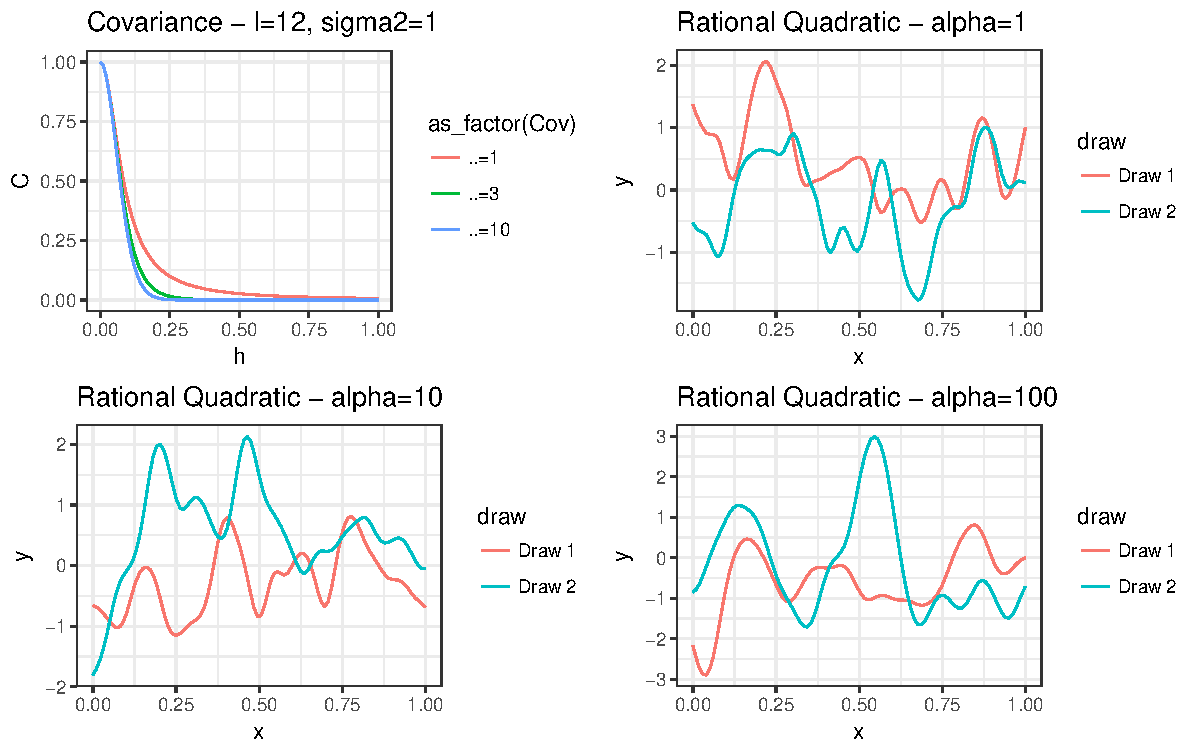
\includegraphics{Lec14_files/figure-beamer/unnamed-chunk-12-1} \end{center}

\end{frame}

\begin{frame}[t]{Some properties}

\begin{itemize}
\tightlist
\item
  \textbf{Matern Covariance}

  \begin{itemize}
  \tightlist
  \item
    A Gaussian process with Matérn covariance has sample functions that
    are \(\lceil \nu -1\rceil\) times differentiable. \vspace{1mm}
  \item
    When \(\nu = 1/2 + p\) for \(p \in \mathbb{N}^+\) then the Matern
    has a simplified form (product of an exponential and a polynomial of
    order \(p\)). \vspace{1mm}
  \item
    When \(\nu = 1/2\) the Matern is equivalent to the exponential
    covariance. \vspace{1mm}\\
  \item
    As \(\nu \to \infty\) the Matern converges to the square exponential
    covariance.
  \end{itemize}
\end{itemize}

\vspace{2mm}

\begin{itemize}
\tightlist
\item
  \textbf{Rational Quadratic Covariance}

  \begin{itemize}
  \tightlist
  \item
    is a scale mixture (infinite sum) of squared exponential covariance
    functions with different characteristic length-scales (\(l\)).
    \vspace{1mm}
  \item
    As \(\alpha \to \infty\) the rational quadratic converges to the
    square exponential covariance. \vspace{1mm}
  \item
    Has sample functions that are infinitely differentiable for any
    value of \(\alpha\)
  \end{itemize}
\end{itemize}

\end{frame}

\begin{frame}[t]{Spherical Covariance}

\vspace{-5mm} \small
\[ Cov(y_{t_i}, y_{t_j}) = Cov(h = |t_i - t_j|) = \begin{cases}
\sigma^2\left(1 - \frac{3}{2} h \cdot l + \frac{1}{2} (h \cdot l)^3)\right) & \text{if   } 0 < h < 1/l \\
0 & \text{otherwise}
\end{cases}\]

\begin{center}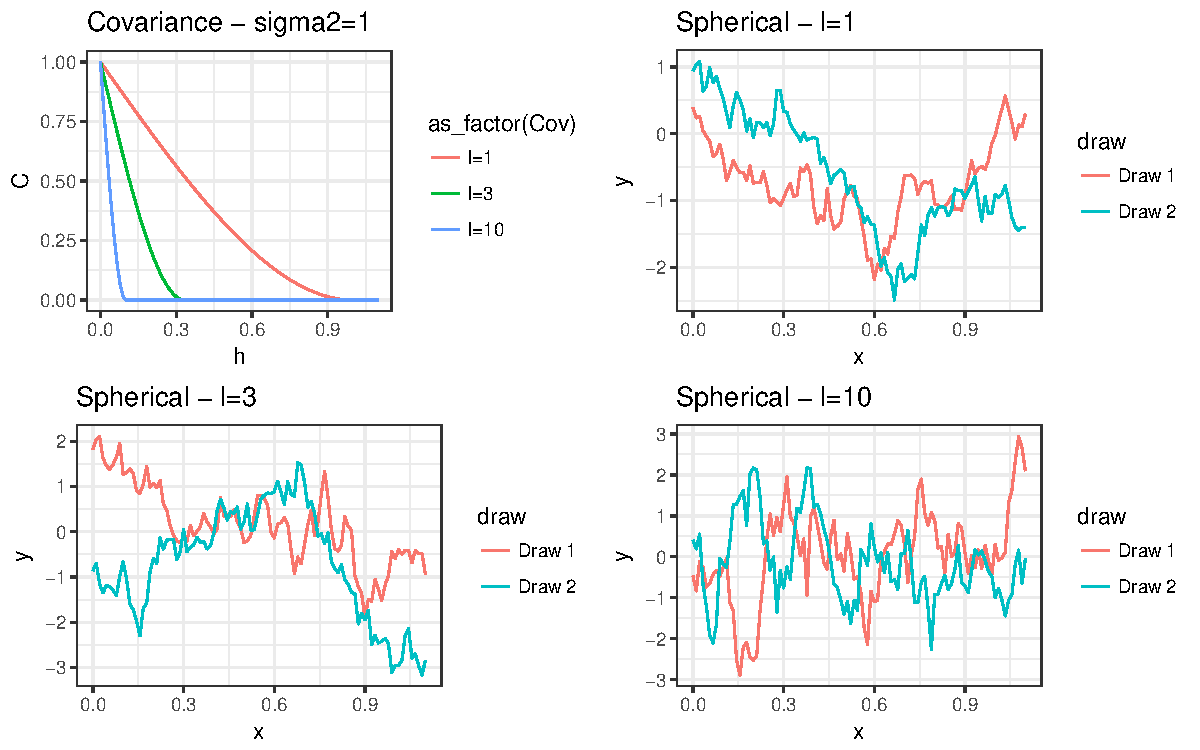
\includegraphics{Lec14_files/figure-beamer/unnamed-chunk-13-1} \end{center}

\end{frame}

\begin{frame}[t]{Periodic Covariance}

\vspace{-5mm}
\[ Cov(y_{t_i}, y_{t_j}) = Cov(h = |t_i - t_j|) = \sigma^2 \exp\left(-2\, l^2 \sin^2\left(\pi\frac{h}{p}\right)\right) \]

\begin{center}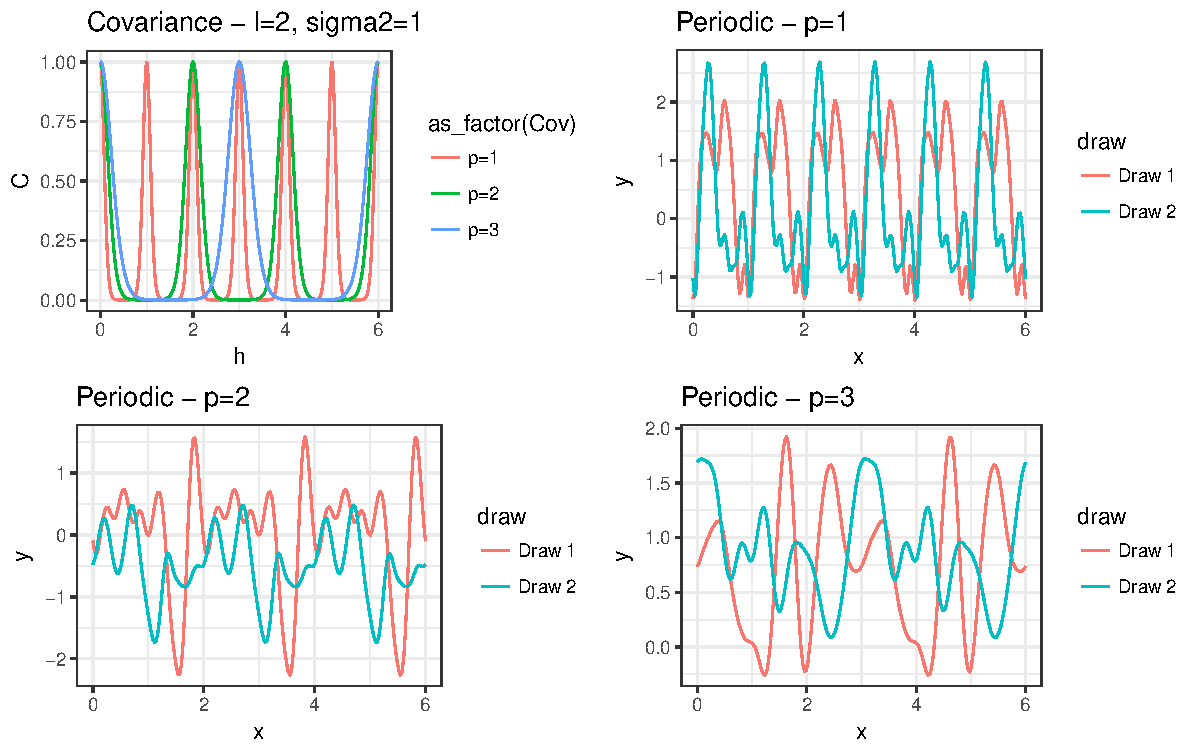
\includegraphics{Lec14_files/figure-beamer/unnamed-chunk-14-1} \end{center}

\end{frame}

\begin{frame}[t]{Linear Covariance}

\vspace{-5mm}
\[ Cov(y_{t_i}, y_{t_j}) = \sigma^2_b + \sigma^2_v~(t_i-c)(t_j-c) \]

\begin{center}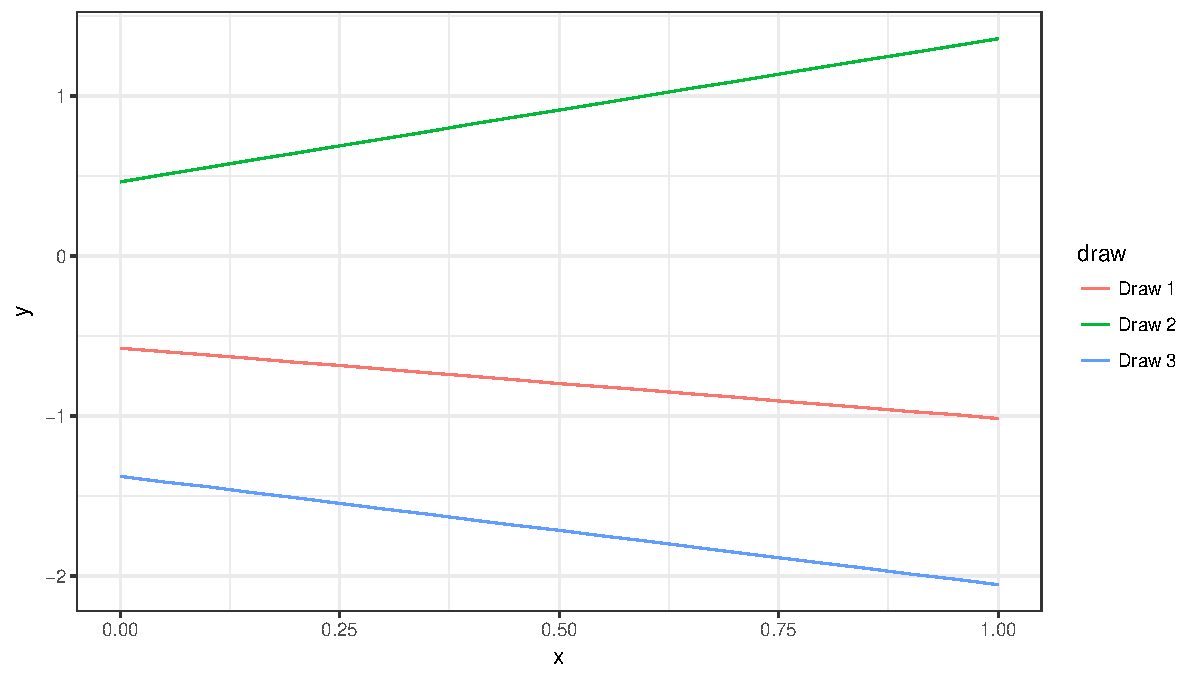
\includegraphics{Lec14_files/figure-beamer/unnamed-chunk-15-1} \end{center}

\end{frame}

\begin{frame}[t]{Combining Covariances}

If we definite two valid covariance functions,
\(Cov_a(y_{t_i}, y_{t_j})\) and \(Cov_b(y_{t_i}, y_{t_j})\) then the
following are also valid covariance functions,

\[
\begin{aligned}
Cov_a(y_{t_i}, y_{t_j}) + Cov_b(y_{t_i}, y_{t_j}) \\
Cov_a(y_{t_i}, y_{t_j}) \times Cov_b(y_{t_i}, y_{t_j})
\end{aligned}
\]

\end{frame}

\begin{frame}[t]{Linear \(\times\) Linear \(\to\) Quadratic}

\vspace{-5mm} \[ Cov_a(y_{t_i}, y_{t_j}) = 1 + 2~(t_i \times t_j) \]
\[ Cov_b(y_{t_i}, y_{t_j}) = 2 + 1~(t_i \times t_j) \]

\begin{center}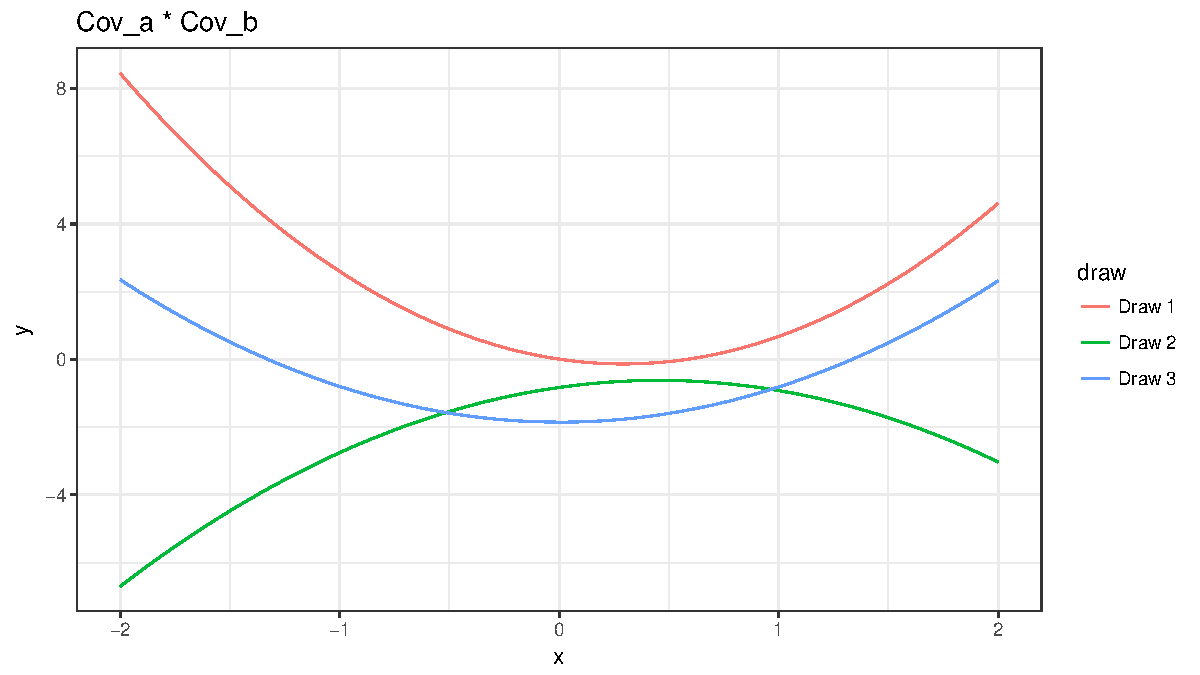
\includegraphics{Lec14_files/figure-beamer/unnamed-chunk-16-1} \end{center}

\end{frame}

\begin{frame}[t]{Linear \(\times\) Periodic}

\vspace{-5mm} \[ Cov_a(y_{t_i}, y_{t_j}) = 1 + 1~(t_i \times t_j) \]
\[ Cov_b(y_{t_i}, y_{t_j}) = Cov(h = |t_i - t_j|) = \exp\left(-2\, \sin^2\left(2\pi\,h\right)\right) \]

\begin{center}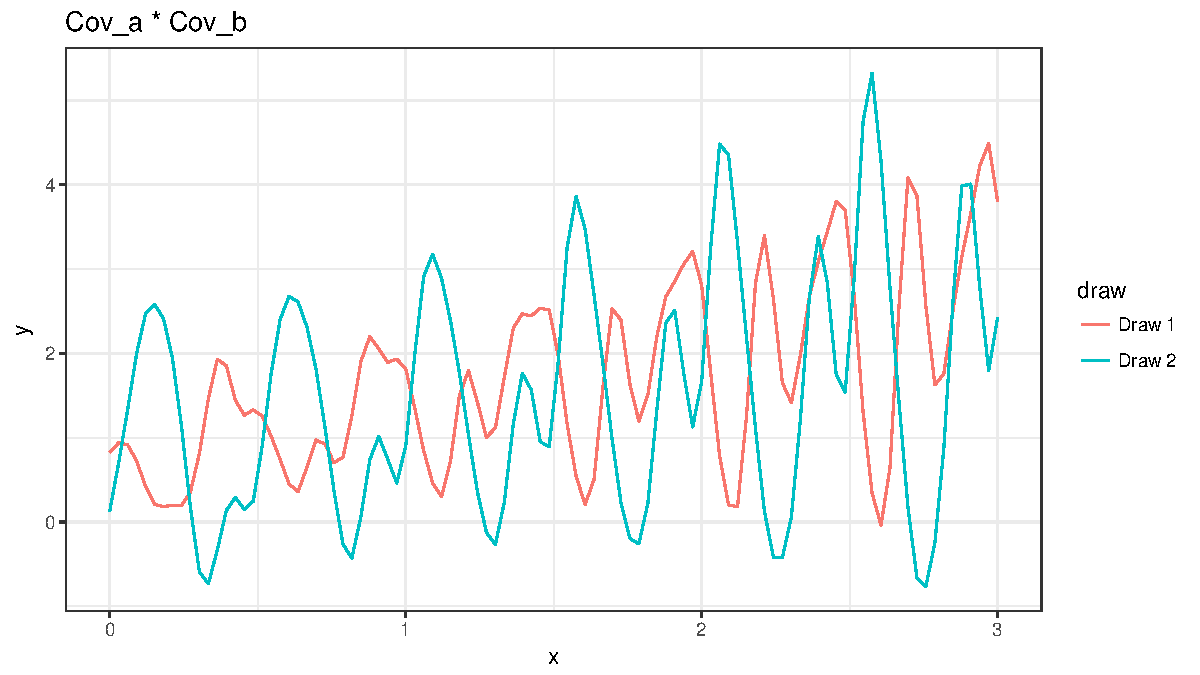
\includegraphics{Lec14_files/figure-beamer/unnamed-chunk-17-1} \end{center}

\end{frame}

\begin{frame}[t]{Linear + Periodic}

\vspace{-5mm} \[ Cov_a(y_{t_i}, y_{t_j}) = 1 + 1~(t_i \times t_j) \]
\[ Cov_b(h = |t_i - t_j|) = \exp\left(-2\, \sin^2\left(2\pi\,h\right)\right) \]

\begin{center}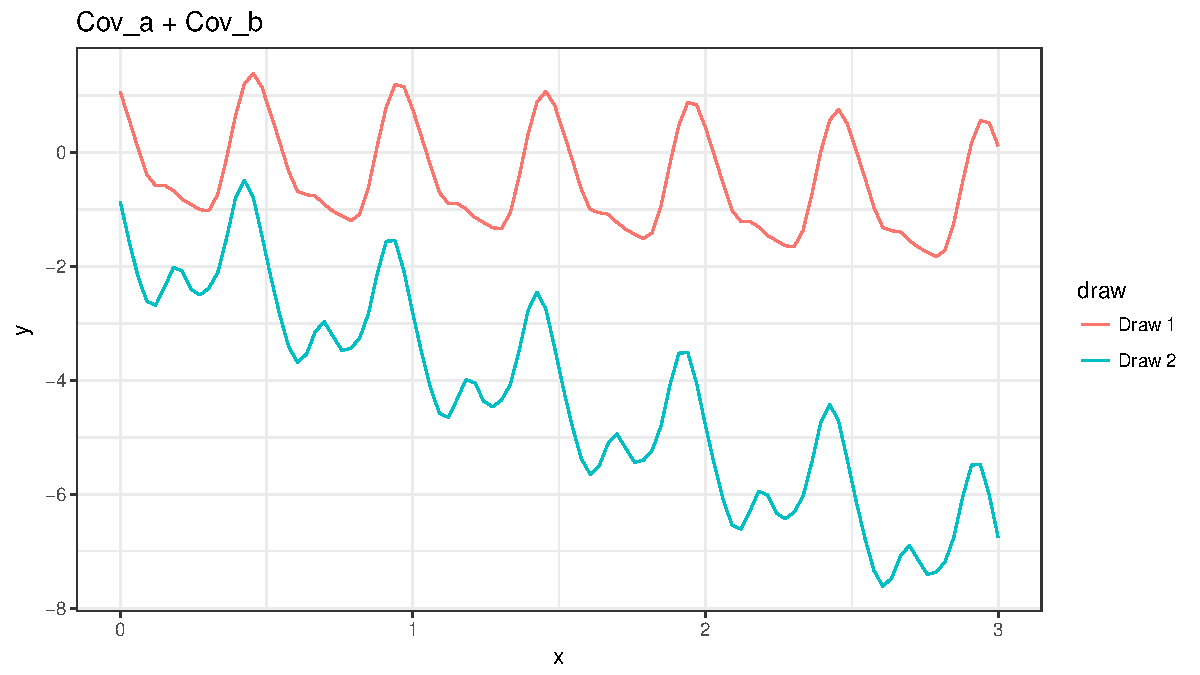
\includegraphics{Lec14_files/figure-beamer/unnamed-chunk-18-1} \end{center}

\end{frame}

\begin{frame}[t]{Sq Exp \(\times\) Periodic \(\to\) Locally Periodic}

\vspace{-5mm} \[ Cov_a(h = |t_i - t_j|) =\exp(-(1/3)h^2) \]
\[ Cov_b(h = |t_i - t_j|) = \exp\left(-2\, \sin^2\left(\pi\,h\right)\right) \]

\begin{center}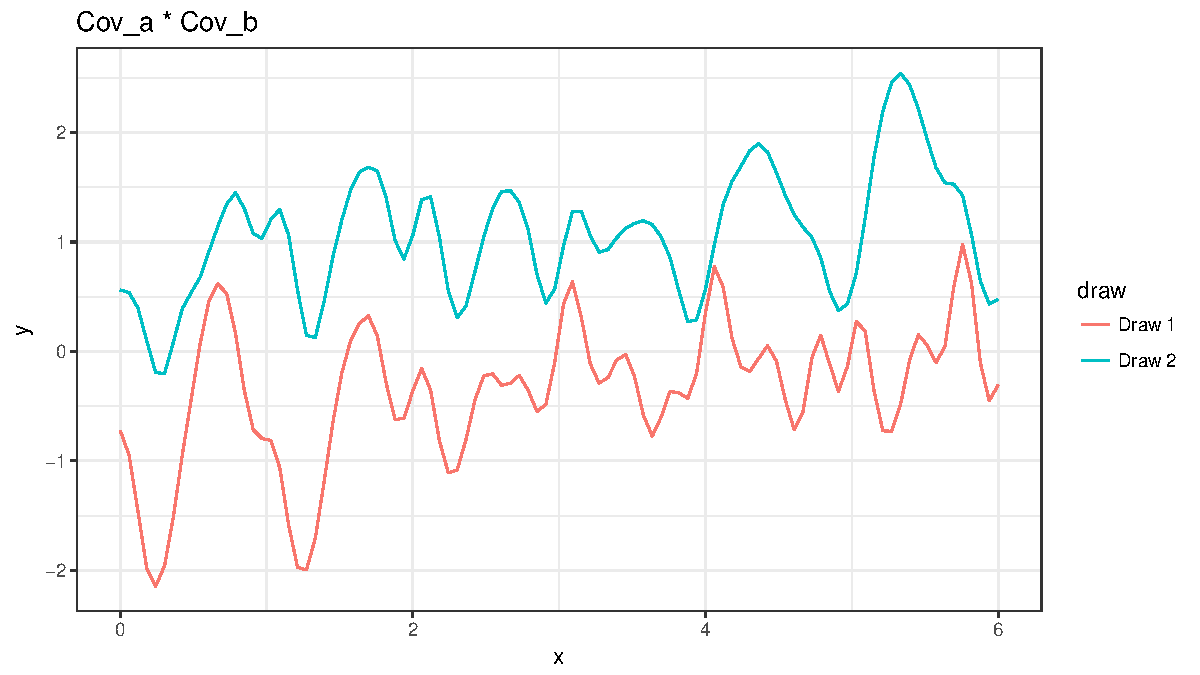
\includegraphics{Lec14_files/figure-beamer/unnamed-chunk-19-1} \end{center}

\end{frame}

\begin{frame}[t]{Sq Exp (short) + Sq Exp (long)}

\vspace{-5mm} \[ Cov_a(h = |t_i - t_j|) = (1/4) \exp(-4\sqrt{3}h^2) \]
\[ Cov_b(h = |t_i - t_j|) = \exp(-(\sqrt{3}/2)h^2) \]

\begin{center}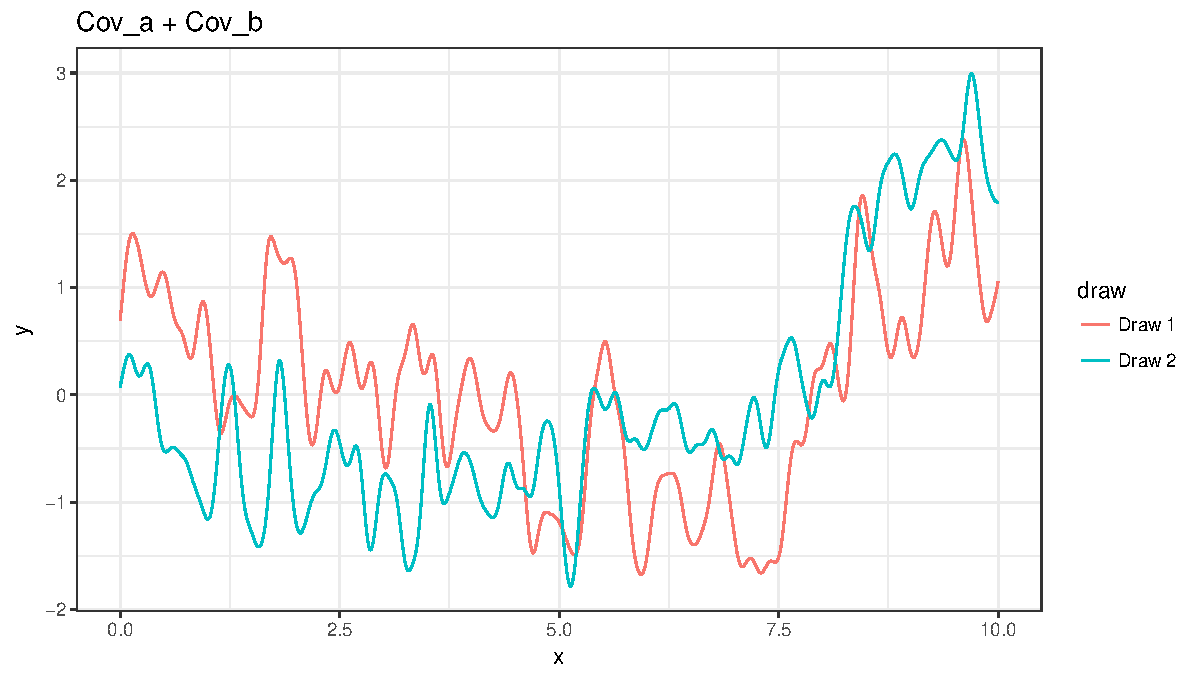
\includegraphics{Lec14_files/figure-beamer/unnamed-chunk-20-1} \end{center}

\end{frame}

\begin{frame}[t]{Sq Exp (short) + Sq Exp (long) (Seen another way)}

\begin{center}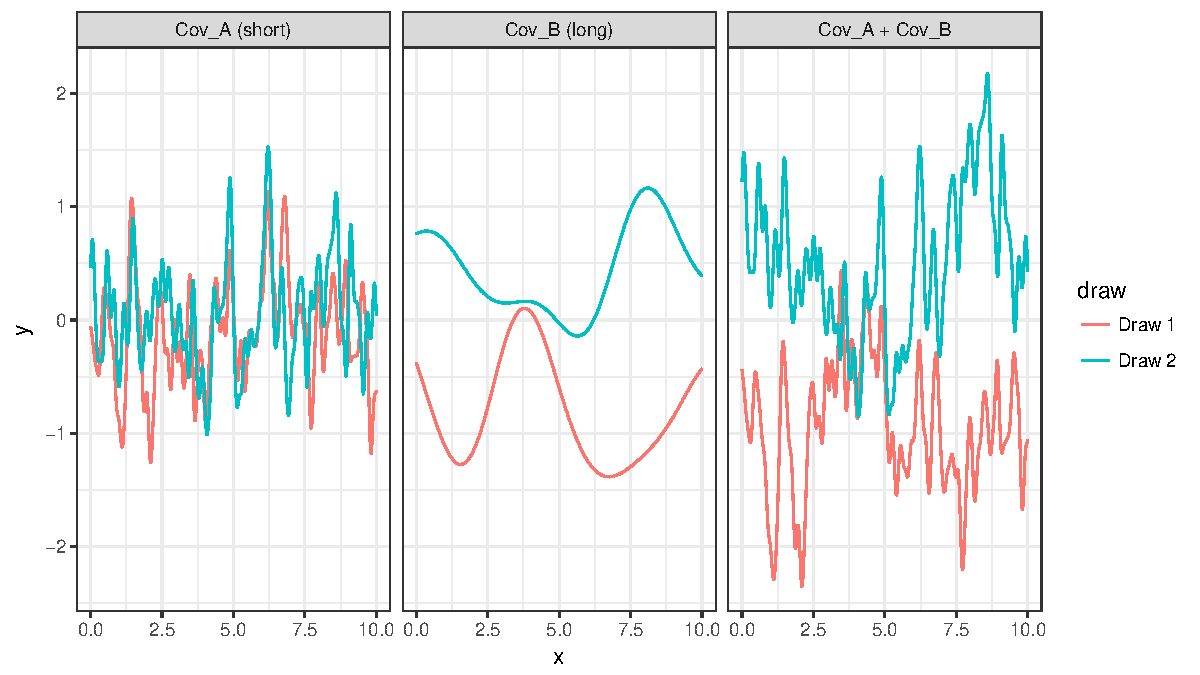
\includegraphics{Lec14_files/figure-beamer/unnamed-chunk-21-1} \end{center}

\end{frame}

\section{BDA3 example}\label{bda3-example}

\begin{frame}{BDA3}

\begin{center}
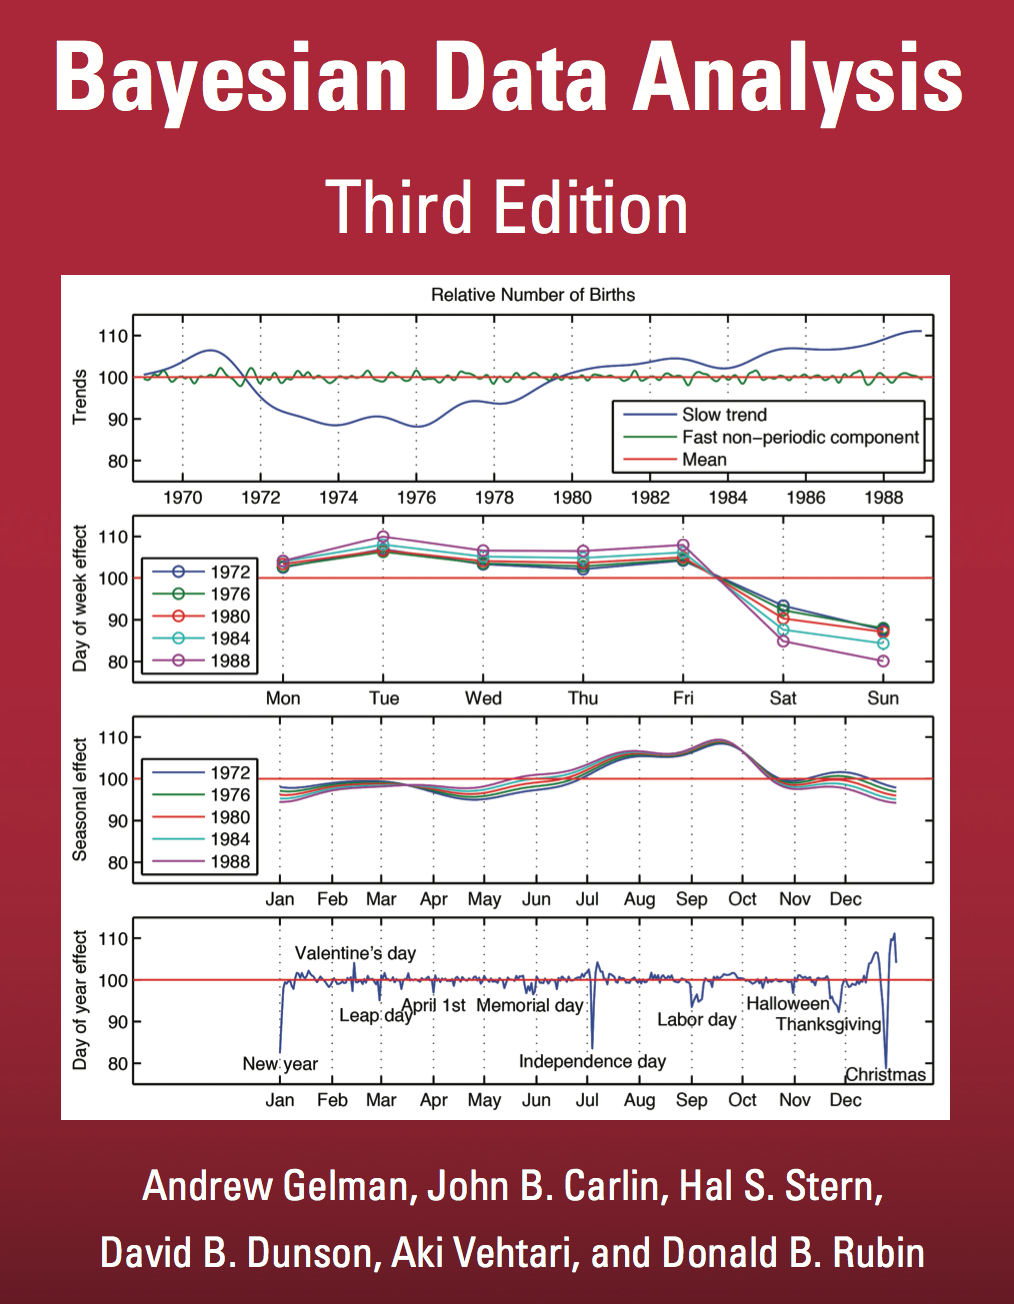
\includegraphics[width=0.7\textwidth]{figs/bda_cover.png} 

$~$

\vspace{-3mm}
\url{http://research.cs.aalto.fi/pml/software/gpstuff/demo_births.shtml}
\end{center}

\end{frame}

\begin{frame}{Births (one year)}

\begin{columns}
\begin{column}{0.5\textwidth}
\begin{center}
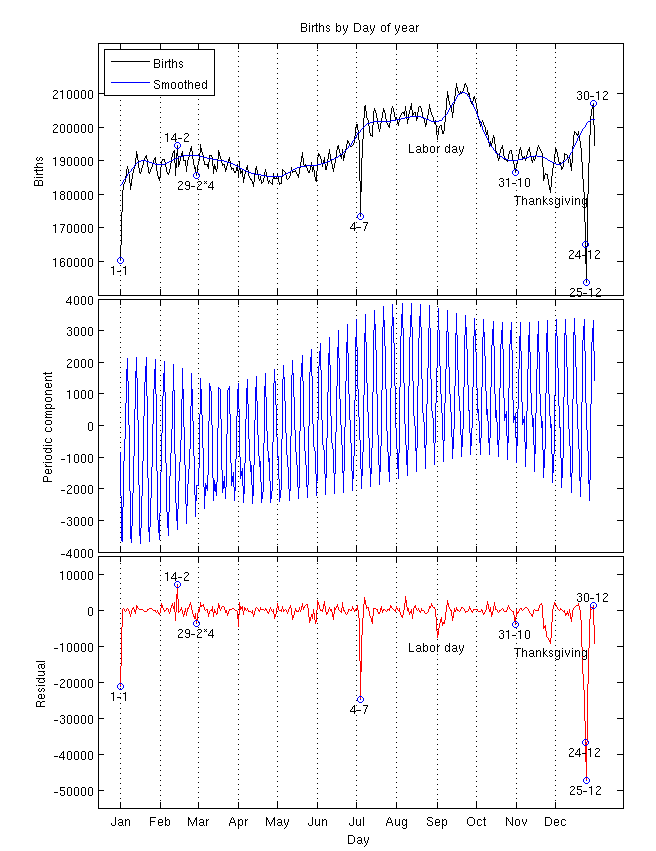
\includegraphics[width=\textwidth]{figs/births_pic1.png}
\end{center}
\end{column}
\begin{column}{0.5\textwidth}

1. Smooth long term trend \\ (\textit{sq exp cov})

\vspace{2mm}

2. Seven day periodic trend with decay (\textit{periodic $\times$ sq exp cov})

\vspace{2mm}

3. Constant mean

\vspace{2mm}

4. Student t observation model

\end{column}
\end{columns}

\end{frame}

\begin{frame}{Births (multiple years)}

\begin{adjustwidth}{-10mm}{-10mm}
\begin{center}
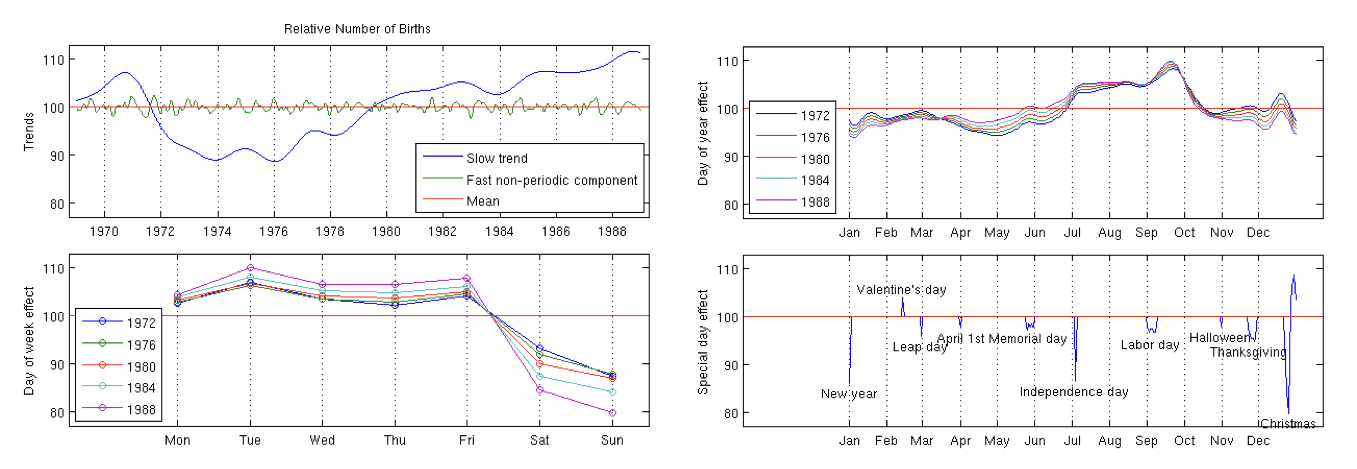
\includegraphics[width=\paperwidth]{figs/births_pic2.png}
\end{center}
\end{adjustwidth}

\vspace{-3mm}

\footnotesize

\begin{enumerate}
\def\labelenumi{\arabic{enumi}.}
\item
  slowly changing trend (\emph{sq exp cov})
\item
  small time scale correlating noise (\emph{sq exp cov})
\item
  7 day periodical component capturing day of week effect
  (\emph{periodic \(\times\) sq exp cov})
\item
  365.25 day periodical component capturing day of year effect
  (\emph{periodic \(\times\) sq exp cov})
\item
  component to take into account the special days and interaction with
  weekends (\emph{linear cov})
\item
  independent Gaussian noise (\emph{nugget cov})
\item
  constant mean
\end{enumerate}

\end{frame}

\end{document}
